\documentclass[10pt,a4paper]{article}
\usepackage[margin=25mm]{geometry}
\usepackage{amsmath,amssymb,amsthm,graphicx,hyperref,stmaryrd,braket}
\title{Probabilistic Boolean circuit axioms are complete for Boolean stochastic maps}
\author{Alessandro Di Giorgio, Pawel Sobocinski, Niels Voorneveld}
\date{doi:10.4230/LIPIcs.CSL.2026.29; CC BY4.0 (official published text and all original diagram images)}
\begin{document}
\maketitle
\noindent\textit{Editorial note.} Copyright Alessandro Di Giorgio, Pawel Sobocinski and Niels Voorneveld; official CSL2026.29 CC BY4.0. Main Theorem11 and its AppendixB Theorem23 restatement count once. All original probabilistic Boolean circuit diagrams and exact printed axiom tags retained; normal-form support and metric applications do not add counts.\par\medskip
\noindent\textit{Allowed standard prerequisites (editorial).}\begin{itemize}
\item Symmetric monoidal/Markov-category coherence, finite probability distributions and stochastic maps. Original Section2 and bibliography, with full current probabilistic-choice axioms and all current normal-form constructions retained. No metric/enrichment or external new-core proof is needed for selected completeness target.
\end{itemize}\medskip

% BEGIN S2
 
\par\medskip\noindent\textbf{2 Symmetric Monoidal Categories as Resource Theories}\par
 
% BEGIN S2.p1
 
In this section we give a brief introduction to symmetric monoidal categories (SMCs) and their associated graphical calculus [13, 23, 22] in terms of resource theories, following [6].\par
 
% END S2.p1
 
% BEGIN S2.p2
 
The basic data consists of objects $A,B,C,\ldots$ that we think of as types of resources, and morphisms $f\colon A\to B$, which we think of as transformations that convert a resource of type $A$ into one of type $B$. Morphisms can be composed sequentially: given $f\colon A\to B$ and $g\colon B\to C$, their composite $f;g\colon A\to C$ represents performing $f$ followed by $g$.\par
 
% END S2.p2
 
% BEGIN S2.p3
 
The monoidal product $\otimes$ lets us express having two resources at once – so $A\otimes C$ means having both $A$ and $C$ – and it extends to morphisms too: given $f\colon A\to B$ and $g\colon C\to D$, the morphism $f\otimes g\colon A\otimes C\to B\otimes D$ describes applying $f$ and $g$ in parallel. There is also a void resource $I$ that acts neutrally under combination: $A\otimes I=A$.\par
 
% END S2.p3
 
% BEGIN S2.p4
 
These ideas are captured visually using the graphical calculus of string diagrams. A resource type $A$ is drawn as a wire $\begin{matrix}
\includegraphics[height=4.375pt]{graphic-001.png}\end{matrix}$, and a transformation $f\colon A_{1}\otimes\ldots\otimes A_{n}\to B_{1}\otimes\ldots\otimes B_{m}$ is represented by a box $\begin{matrix}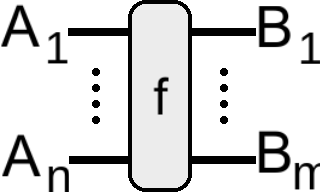
\includegraphics[height=12.5pt]{graphic-002.png}\end{matrix}$ with $n$ input wires on the left and $m$ output wires on the right. Composition of morphisms is shown by connecting boxes in sequence $\begin{matrix}
\includegraphics[height=4.375pt]{graphic-003.png}\end{matrix}$, while the monoidal product corresponds to placing them side-by-side $\begin{matrix}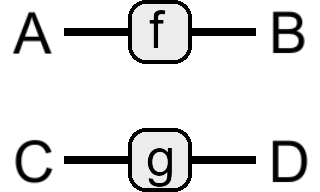
\includegraphics[height=12.5pt]{graphic-004.png}\end{matrix}$. The void resource $I$ corresponds to no wires at all – i.e., the empty diagram.\par
 
% END S2.p4
 
% BEGIN S2.p5
 
Resources can also be swapped according to the symmetry $\chi_{A,B}\colon A\otimes B\to B\otimes A$, which is represented by a crossing of wires $\begin{matrix}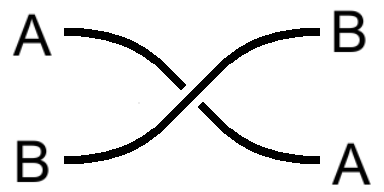
\includegraphics[height=12.5pt]{graphic-005.png}\end{matrix}$.\par
 
% END S2.p5
 
% BEGIN S2.p6
 
Diagrams are subject to the axioms of symmetric monoidal categories (SMCs). However, note that equational reasoning in this setting amounts to deformation of diagrams without changing their topology. For example, naturality of symmetry amounts to sliding a box past a crossing of wires, illustrated as $\begin{matrix}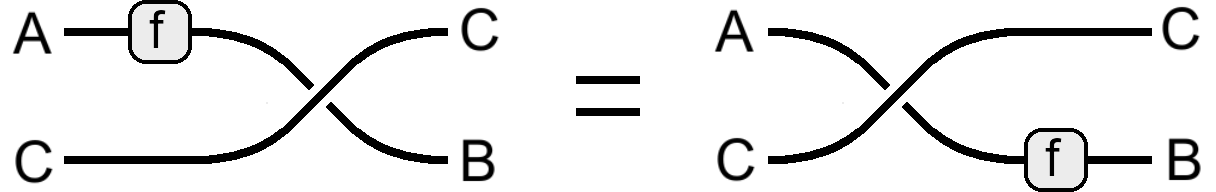
\includegraphics[height=12.5pt]{graphic-006.png}\end{matrix}$.\par
 
% END S2.p6
 
% BEGIN S2.p7
 
In the next section, where we introduce the parametric iteration construction, it will be convenient to explicitly track both the combination of resources via the monoidal product and the void resource. Therefore, following [4], we extend the graphical calculus with operations that introduce $\begin{matrix}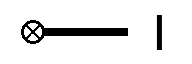
\includegraphics[height=4.375pt]{graphic-007.png}\end{matrix}$ and discard $\begin{matrix}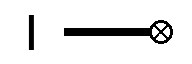
\includegraphics[height=4.375pt]{graphic-008.png}\end{matrix}$ the void resource, as well as split $\begin{matrix}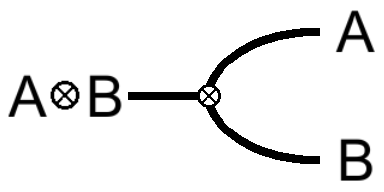
\includegraphics[height=12.5pt]{graphic-009.png}\end{matrix}$ and combine $\begin{matrix}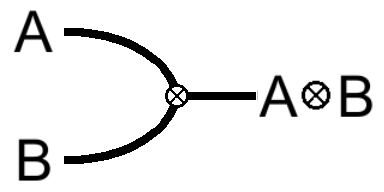
\includegraphics[height=12.5pt]{graphic-010.png}\end{matrix}$ resources. These operations are subject to the expected equations determined by the properties of the monoidal product.\par
 
% END S2.p7
 
% BEGIN S2.p8
 
Finally, note that all monoidal categories considered in this paper are taken to be strict, as justified by Mac Lane’s strictification theorem [18].\par
 
% END S2.p8
 
% END S2


% BEGIN S4
 
\par\medskip\noindent\textbf{4 Reasoning with Probabilities and Distances}\par
 
% BEGIN S4.p1
 
To model richer computational behaviors, we consider symmetric monoidal categories with additional properties and structure. In particular, for probabilistic computations, we focus on metric-enriched symmetric monoidal categories and Markov categories [10].\par
 
% END S4.p1
 
% BEGIN S4.F1
  
\par  \quad  
\begin{center}\resizebox{0.98\linewidth}{!}{$\begin{array}[]{c@{\quad}c@{\quad}c}\begin{matrix}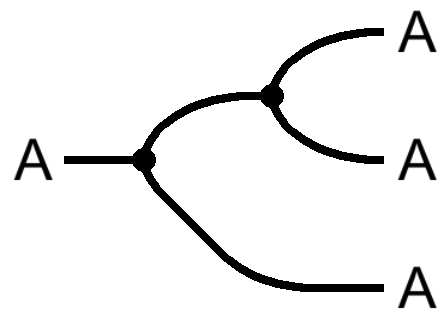
\includegraphics[height=20.0pt]{graphic-011.png}\end{matrix}\stackrel{{\scriptstyle(\blacktriangleleft\text{-as})}}{{=}}\begin{matrix}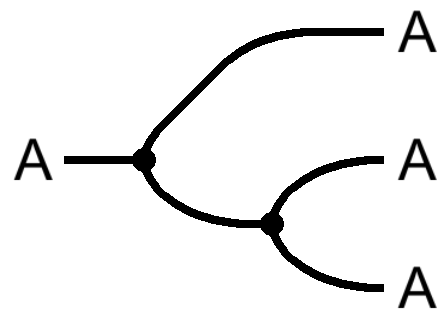
\includegraphics[height=20.0pt]{graphic-012.png}\end{matrix}&\begin{matrix}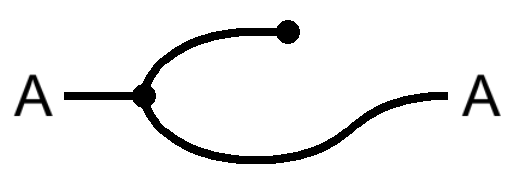
\includegraphics[height=12.5pt]{graphic-013.png}\end{matrix}\stackrel{{\scriptstyle(\blacktriangleleft\text{-un})}}{{=}}\begin{matrix}
\includegraphics[height=4.375pt]{graphic-014.png}\end{matrix}&\begin{matrix}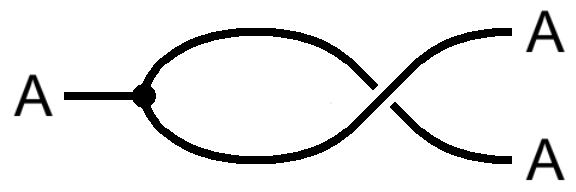
\includegraphics[height=12.5pt]{graphic-015.png}\end{matrix}\stackrel{{\scriptstyle(\blacktriangleleft\text{-co})}}{{=}}\begin{matrix}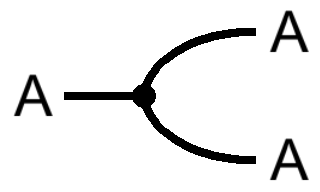
\includegraphics[height=12.5pt]{graphic-016.png}\end{matrix}\\
&\begin{matrix}
\includegraphics[height=4.375pt]{graphic-017.png}\end{matrix}\stackrel{{\scriptstyle(!\text{-nat})}}{{=}}\begin{matrix}
\includegraphics[height=4.375pt]{graphic-018.png}\end{matrix}&\\
\hline\multicolumn{3}{c}{\begin{array}[]{c@{\quad}c@{\quad}c@{\quad}c}\begin{matrix}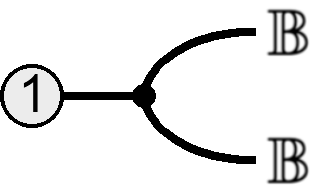
\includegraphics[height=12.5pt]{graphic-019.png}\end{matrix}\stackrel{{\scriptstyle(1\text{-det})}}{{=}}\begin{matrix}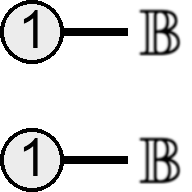
\includegraphics[height=12.5pt]{graphic-020.png}\end{matrix}&\begin{matrix}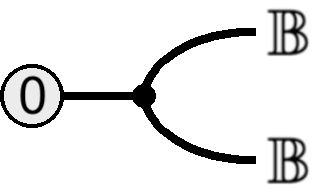
\includegraphics[height=12.5pt]{graphic-021.png}\end{matrix}\stackrel{{\scriptstyle(0\text{-det})}}{{=}}\begin{matrix}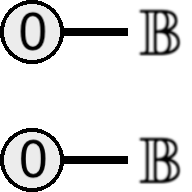
\includegraphics[height=12.5pt]{graphic-022.png}\end{matrix}&\begin{matrix}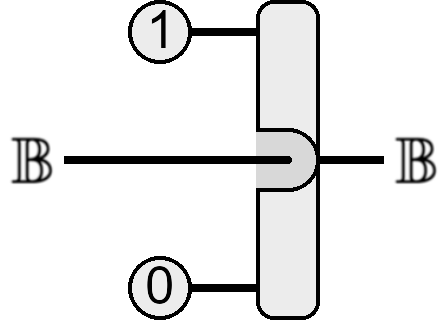
\includegraphics[height=20.0pt]{graphic-023.png}\end{matrix}\stackrel{{\scriptstyle(\phi\text{-B})}}{{=}}\begin{matrix}
\includegraphics[height=4.375pt]{graphic-024.png}\end{matrix}&\begin{matrix}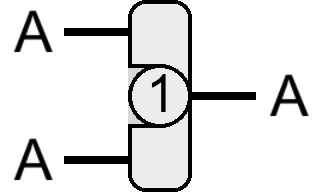
\includegraphics[height=12.5pt]{graphic-025.png}\end{matrix}\stackrel{{\scriptstyle(\phi\text{-1})}}{{=}}\begin{matrix}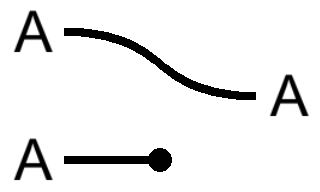
\includegraphics[height=12.5pt]{graphic-026.png}\end{matrix}\end{array}}\\[15.0pt]
\begin{matrix}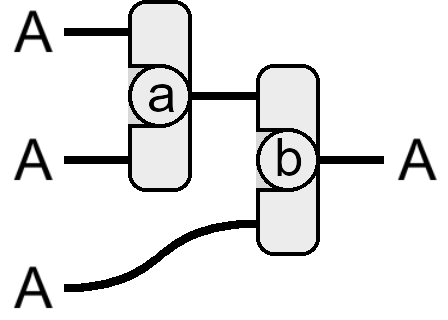
\includegraphics[height=20.0pt]{graphic-027.png}\end{matrix}\stackrel{{\scriptstyle(\phi\text{-as})}}{{=}}\begin{matrix}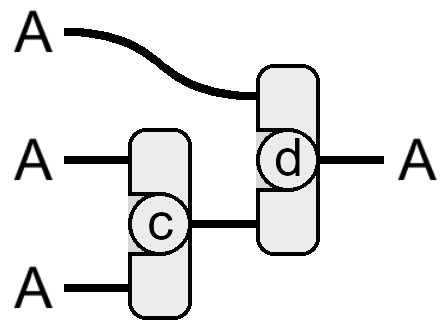
\includegraphics[height=20.0pt]{graphic-028.png}\end{matrix}&\begin{matrix}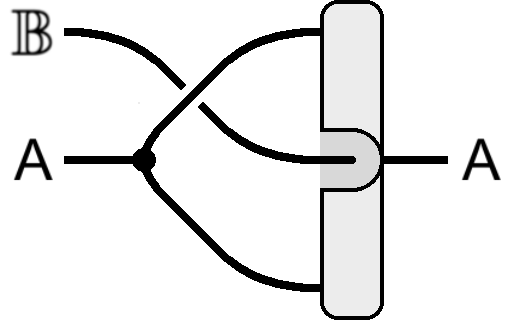
\includegraphics[height=20.0pt]{graphic-029.png}\end{matrix}\stackrel{{\scriptstyle(\phi\text{-id})}}{{=}}\begin{matrix}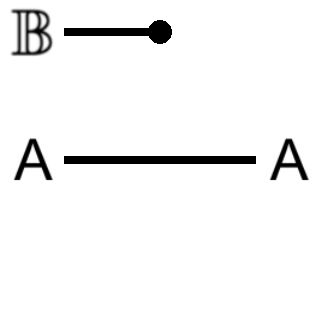
\includegraphics[height=20.0pt]{graphic-030.png}\end{matrix}&\begin{matrix}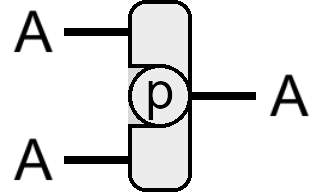
\includegraphics[height=12.5pt]{graphic-031.png}\end{matrix}\stackrel{{\scriptstyle(\phi\text{-co})}}{{=}}\begin{matrix}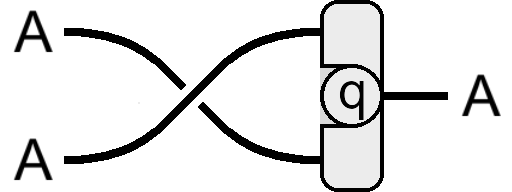
\includegraphics[height=12.5pt]{graphic-032.png}\end{matrix}\\[15.0pt]
\begin{matrix}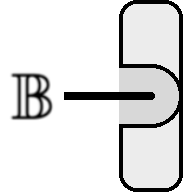
\includegraphics[height=12.5pt]{graphic-033.png}\end{matrix}\stackrel{{\scriptstyle(\phi_I)}}{{=}}\begin{matrix}
\includegraphics[height=4.375pt]{graphic-034.png}\end{matrix}&\begin{matrix}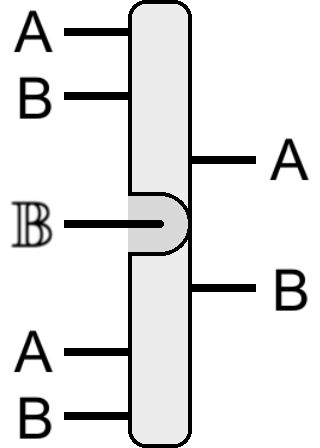
\includegraphics[height=28.125pt]{graphic-035.png}\end{matrix}\stackrel{{\scriptstyle(\phi_{\otimes})}}{{=}}\begin{matrix}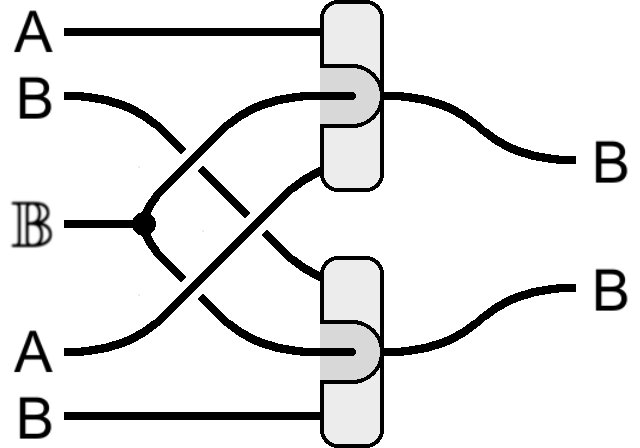
\includegraphics[height=28.125pt]{graphic-036.png}\end{matrix}&\begin{matrix}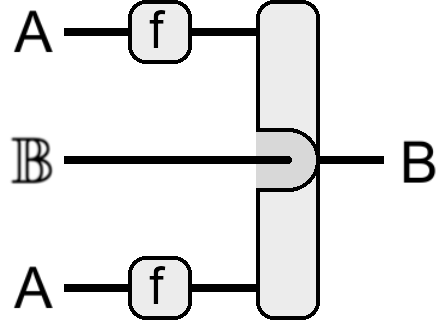
\includegraphics[height=20.0pt]{graphic-037.png}\end{matrix}\stackrel{{\scriptstyle(\phi\text{-nat})}}{{=}}\begin{matrix}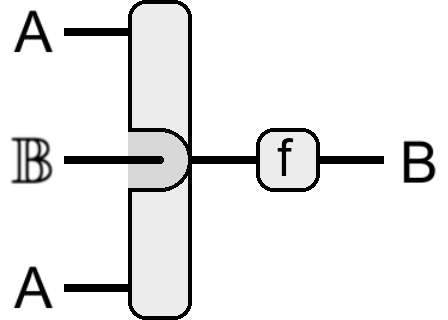
\includegraphics[height=20.0pt]{graphic-038.png}\end{matrix}\end{array}$}\end{center}
\quad  \quad  
  
Figure 1: Axioms for Markov categories (top) and probabilistic choice (bottom). Here $f\colon A\to B$, $q=1-p$, $c=\frac{(1-a)b}{1-ab}$ and $d=ab$.\par
 
% END S4.F1
 
% BEGIN Thmtheorem9
 
\par\medskip\noindent\textbf{Definition 9.}\par
 
% BEGIN Thmtheorem9.p1
 
A Markov category with probabilistic choice is a symmetric monoidal category equipped with operations $!_{A}\colon A\to I$, $\blacktriangleleft_{A}\colon A\to A\otimes A$, $\langle p\rangle\colon I\to\mathbb{B}$ and $\phi_{A}\colon A\otimes\mathbb{B}\otimes A\to A$, represented in string diagrams, respectively, as\par
 
$\begin{matrix}
\includegraphics[height=4.375pt]{graphic-018.png}\end{matrix}$ $\begin{matrix}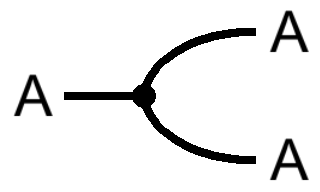
\includegraphics[height=12.5pt]{graphic-016.png}\end{matrix}$ $\begin{matrix}
\includegraphics[height=4.375pt]{graphic-039.png}\end{matrix}$ $\begin{matrix}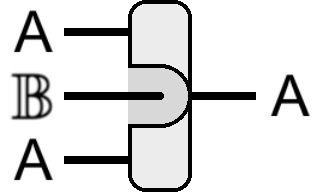
\includegraphics[height=12.5pt]{graphic-040.png}\end{matrix}$\par
 
where $p\in[0,1]$, $\mathbb{B}$ is a designated object and $A$ is any object, and such that the axioms in Figure 1 hold. That is:\par
  
\par\noindent  $\blacksquare$ 
% BEGIN S4.I1.i1.p1
 
$(\blacktriangleleft_{A},!_{A})$ is a cocommutative comonoid, that is $\blacktriangleleft_{A}$ is associative ($\blacktriangleleft\text{-as}$), cocommutative ($\blacktriangleleft\text{-co}$) and $!_{A}$ is the unit ($\blacktriangleleft\text{-un}$),\par
 
% END S4.I1.i1.p1
 
 
\par\noindent  $\blacksquare$ 
% BEGIN S4.I1.i2.p1
 
$\blacktriangleleft_{A}$ and $!_{A}$ are coherent with the monoidal structure,\par
 
% END S4.I1.i2.p1
 
 
\par\noindent  $\blacksquare$ 
% BEGIN S4.I1.i3.p1
 
$!_{A}$ is natural ($!\text{-nat}$),\par
 
% END S4.I1.i3.p1
 
 
\par\noindent  $\blacksquare$ 
% BEGIN S4.I1.i4.p1
 
$\langle 1\rangle$ and $\langle 0\rangle$ are deterministic (($1\text{-det}$) and ($0\text{-det}$)),\par
 
% END S4.I1.i4.p1
 
 
\par\noindent  $\blacksquare$ 
% BEGIN S4.I1.i5.p1
 
$\phi_{A}$ is coherent with the monoidal structure (($\phi_I$) and ($\phi_{\otimes}$)),\par
 
% END S4.I1.i5.p1
 
 
\par\noindent  $\blacksquare$ 
% BEGIN S4.I1.i6.p1
 
$\phi_{A}$ is natural in $A$ ($\phi\text{-nat}$),\par
 
% END S4.I1.i6.p1
 
 
\par\noindent  $\blacksquare$ 
% BEGIN S4.I1.i7.p1
 
$\phi_{A}^{p}$–where $\phi_{A}^{p}$ is $\begin{matrix}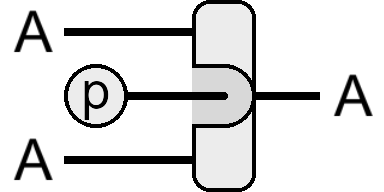
\includegraphics[height=12.5pt]{graphic-041.png}\end{matrix}$, often simply $\begin{matrix}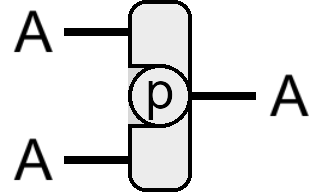
\includegraphics[height=12.5pt]{graphic-042.png}\end{matrix}$–is a convex algebra, that is, $\phi^{p}_{A}$ is idempotent ($\phi\text{-id}$) and satisfies parametric associativity ($\phi\text{-as}$) and commutativity ($\phi\text{-co}$),\par
 
% END S4.I1.i7.p1
 
 
\par\noindent  $\blacksquare$ 
% BEGIN S4.I1.i8.p1
 
$\phi$ and $\langle 1\rangle$, $\langle 0\rangle$ interact via ($\phi\text{-B}$) and ($\phi\text{-1}$).\par
 
% END S4.I1.i8.p1
 
  
% END Thmtheorem9.p1
 
% END Thmtheorem9
 
% BEGIN S4.p2
 
The $\mathbb{B}$ represents the type of two bit values, $1$ and $0$. $\langle p\rangle$ describes a weighted coin flip, which has a chance of $p$ of producing $1$, and a chance of $1-p$ of producing $0$. The $\phi$ represents an if-gate, choosing between two results of the same type using a bit as an argument.\par
 
% END S4.p2
 
% BEGIN S4.F2
  
\par  \quad  \[\begin{array}[]{c@{\qquad\qquad}c}\begin{matrix}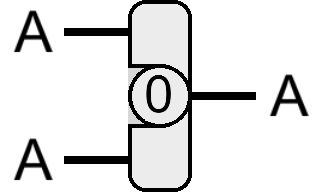
\includegraphics[height=12.5pt]{graphic-043.png}\end{matrix}\stackrel{{\scriptstyle(\phi\text{-0})}}{{=}}\begin{matrix}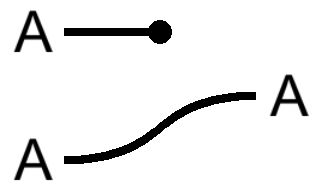
\includegraphics[height=12.5pt]{graphic-044.png}\end{matrix}&\begin{matrix}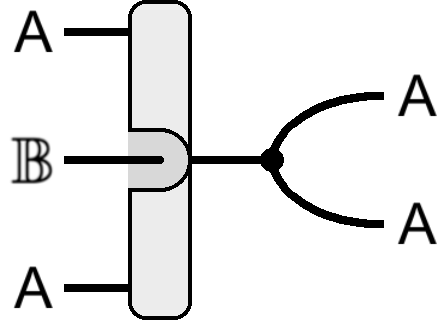
\includegraphics[height=20.0pt]{graphic-045.png}\end{matrix}\stackrel{{\scriptstyle(\phi\text{-det})}}{{=}}\begin{matrix}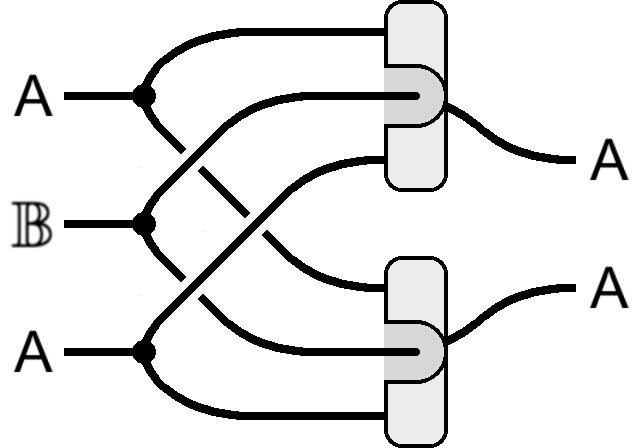
\includegraphics[height=28.125pt]{graphic-046.png}\end{matrix}\\
\begin{matrix}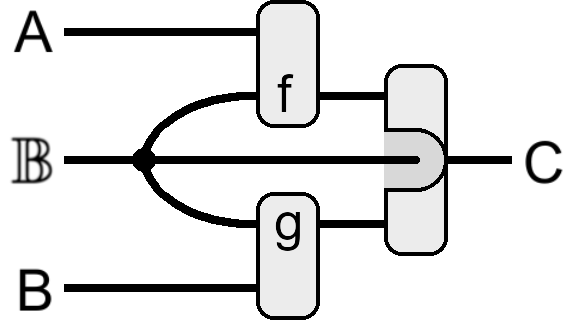
\includegraphics[height=20.0pt]{graphic-047.png}\end{matrix}\stackrel{{\scriptstyle(\mathbb{B}\text{-split})}}{{=}}\begin{matrix}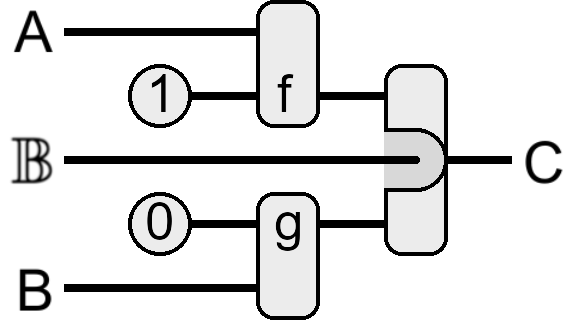
\includegraphics[height=20.0pt]{graphic-048.png}\end{matrix}&\begin{matrix}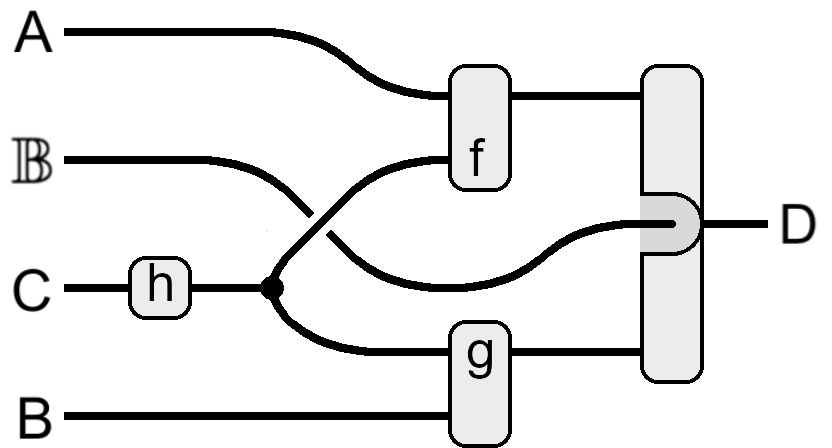
\includegraphics[height=28.125pt]{graphic-049.png}\end{matrix}\stackrel{{\scriptstyle(\phi\text{-distr})}}{{=}}\begin{matrix}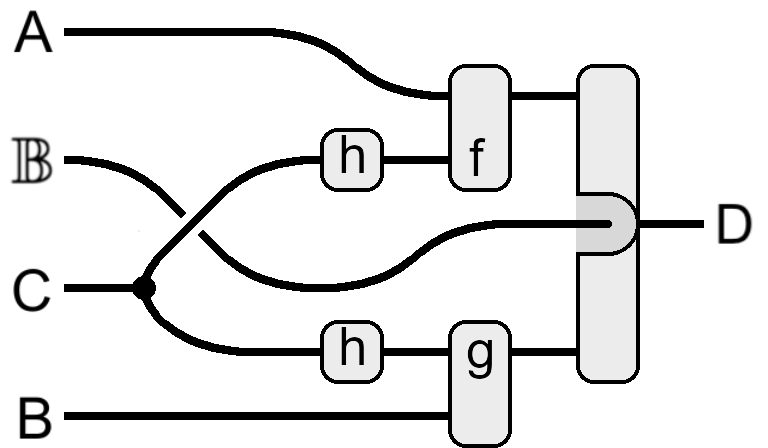
\includegraphics[height=28.125pt]{graphic-050.png}\end{matrix}\end{array}\]\quad  \quad  
  
Figure 2: Derived laws for Markov categories with probabilistic choice.\par
 
% END S4.F2
 
% BEGIN Thmtheorem10
 
\par\medskip\noindent\textbf{Lemma 10.}\par
 
% BEGIN Thmtheorem10.p1
 
The laws in Figure 2 hold in any Markov category with probabilistic choice.\par
 
% END Thmtheorem10.p1
 
% END Thmtheorem10
 
% BEGIN S4.SS0.SSS0.P0.SPx1
 
\par\medskip\noindent\textbf{Proof.}\par
 
% BEGIN S4.SS0.SSS0.P0.SPx1.p1
 
We give a proof only for ($\phi\text{-det}$), the rest can be found in Appendix C.\par
  
\par  \quad  \[\begin{matrix}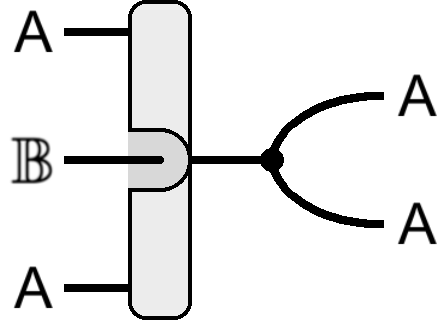
\includegraphics[height=20.0pt]{graphic-045.png}\end{matrix}\stackrel{{\scriptstyle(\phi\text{-nat})}}{{=}}\begin{matrix}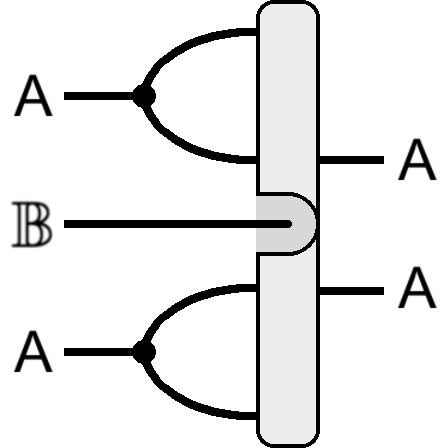
\includegraphics[height=28.125pt]{graphic-051.png}\end{matrix}\stackrel{{\scriptstyle(\phi_{\otimes})}}{{=}}\begin{matrix}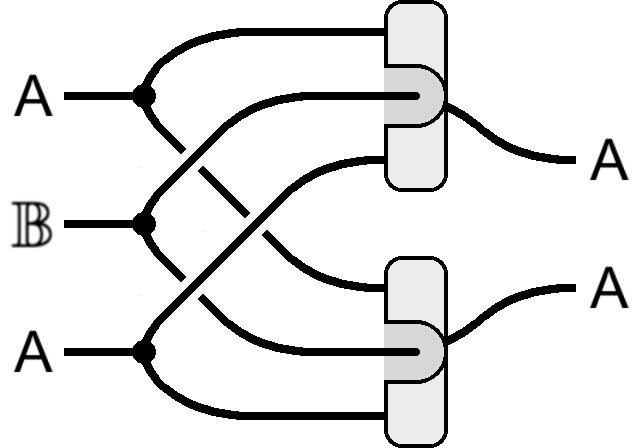
\includegraphics[height=28.125pt]{graphic-046.png}\end{matrix}\]\quad  \quad  
  
$\hfill\blacktriangleleft$ Our leading example of Markov category with probabilistic choice is $\mathsf{FinStoch}$, the category of sets and stochastic maps. Objects are sets and morphisms $f\colon A\to B$ are functions $A\to\mathcal{D}B$ mapping each $a\in A$ to a finitely-supported discrete probability distribution over $B$. We represent a distribution as a function $v:A\to[0,1]$ with finite support $\texttt{supp}(v):=\{a\in A\mid v(a)>0\}$ and such that $\sum_{a\in A}v(a)=1$, or, alternatively, as a formal sum $\sum_{i}{p_{i}\ket{a_{i}}}$, where the $\ket{\cdot}$ notation is used to separate the elements $a_{i}\in A$ from their associated probability $p_{i}\in[0,1]$.\par
 
% END S4.SS0.SSS0.P0.SPx1.p1
 
% BEGIN S4.SS0.SSS0.P0.SPx1.p2
 
We write $f(b|a)$ for $f(a)(b)$, representing the probability that $f$ returns $b$, given $a$. For two stochastic maps $f\colon A\to B,g\colon B\to C$, their composition is defined by summing over the middle variable, i.e. $(f;g)(c\mid a):=\sum_{b\in B}g(c\mid b)f(b\mid a)$. Identities $id_{A}\colon A\to A$ map each $a\in A$ to the Dirac distribution at $a$, i.e. $id_{A}(a):=\ket{a}$.\par
 
% END S4.SS0.SSS0.P0.SPx1.p2
 
% BEGIN S4.SS0.SSS0.P0.SPx1.p3
 
Given two distributions $v\in\mathcal{D}A$ and $u\in\mathcal{D}B$, their product $v\otimes w\in\mathcal{D}{(A\times B)}$ is given by $v\otimes u(a,b):=v(a)u(b)$. This yields a symmetric monoidal structure, with the monoidal product $\otimes$ being the cartesian product of sets $\times$ on objects and with monoidal unit the singleton set $I:=\{\bullet\}$. For arrows $f\colon A\to B$ and $g\colon C\to D$, $f\otimes g\colon A\otimes C\to B\otimes D$ is defined as $f\otimes g(b,d|a,c):=f(b|a)g(d|c)$, and symmetries $\chi_{A,B}\colon A\otimes B\to B\otimes A$ as $\chi_{A,B}(a,b):=\ket{b}\otimes\ket{a}$.\par
 
% END S4.SS0.SSS0.P0.SPx1.p3
 
% BEGIN S4.SS0.SSS0.P0.SPx1.p4
 
The comonoid structure is given by $\blacktriangleleft_{A}(a):=\ket{a}\otimes\ket{a}$ and $!_{A}(a):=\ket{\bullet}$, while for the probabilistic choice structure we take as choice object the set of Booleans $\{1,0\}$ and, for any $p\in[0,1]$, we define $\langle p\rangle\colon\{\bullet\}\to\{1,0\}$ as $\langle p\rangle(\bullet):=p\ket{1}+(1-p)\ket{0}$ and $\phi_{A}\colon A\otimes\{1,0\}\otimes A\to A$ as $\phi_{A}(a,1,b):=\ket{a}$ and $\phi_{A}(a,0,b):=\ket{b}$. Note that $\phi^{p}_{A}(a,b)=p\ket{a}+(1-p)\ket{b}$.\par
 
% END S4.SS0.SSS0.P0.SPx1.p4
 
% BEGIN S4.SS0.SSS0.P0.SPx1.p5
 
Throughout the rest of the paper we will work in $\mathsf{FinStoch}_{\{1,0\}}$, the subcategory of $\mathsf{FinStoch}$ consisting of stochastic maps between sets that are powers of the booleans. The structure of Markov category with probabilistic choice, introduced here, is novel and it offers an alternative presentation of $\mathsf{FinStoch}_{\{1,0\}}$ to the one in [21]. In particular:\par
 
% END S4.SS0.SSS0.P0.SPx1.p5
 
% BEGIN Thmtheorem11
 
\par\medskip\noindent\textbf{Theorem 11.}\par
 
% BEGIN Thmtheorem11.p1
 
the axioms in Figure 1 are complete for $\mathsf{FinStoch}_{\{1,0\}}$.\par
 
% END Thmtheorem11.p1
 
% END Thmtheorem11
 
% BEGIN S4.SS0.SSS0.P0.SPx1.p6
 
The interested reader can find the details in Appendix B.\par
 
% END S4.SS0.SSS0.P0.SPx1.p6
 
% BEGIN S4.SS0.SSS0.P0.SPx1.p7
 
As an example of diagrammatic reasoning in $\mathsf{FinStoch}_{\{1,0\}}$ we look at the one-time-pad protocol on a single bit. We regard $\langle\frac{1}{2}\rangle\colon I\to\mathbb{B}$ as an operation that produces a randomly generated bit, and the xor $\oplus\colon\mathbb{B}\otimes\mathbb{B}\to\mathbb{B}$, defined below on the left, as an operation that encrypts and decrypts a bit.\par
 
$\begin{matrix}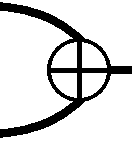
\includegraphics[height=9.375pt]{graphic-052.png}\end{matrix}$ := $\begin{matrix}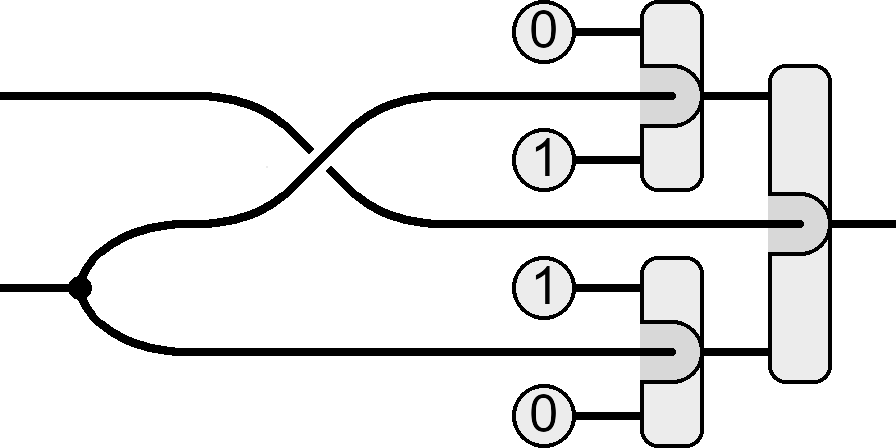
\includegraphics[height=28.125pt]{graphic-053.png}\end{matrix}$ $\begin{matrix}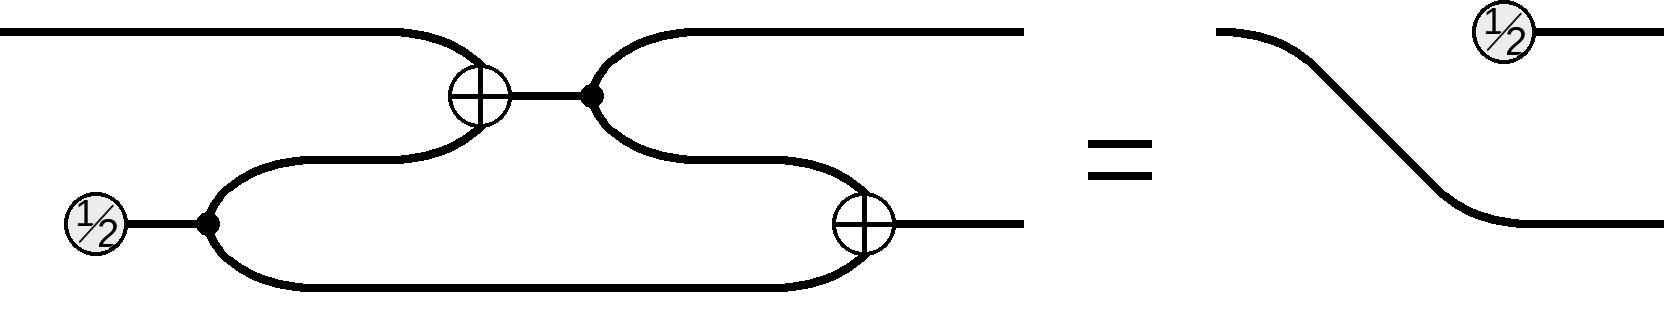
\includegraphics[height=20.0pt]{graphic-054.png}\end{matrix}$\par
 
The equation on the right expresses the correctness of the protocol: encoding and decoding with the same randomly generated bit gets the same result, and that to an adversary the encrypted message looks completely random. We prove correcteness by equational reasoning:\par
 
$\begin{matrix}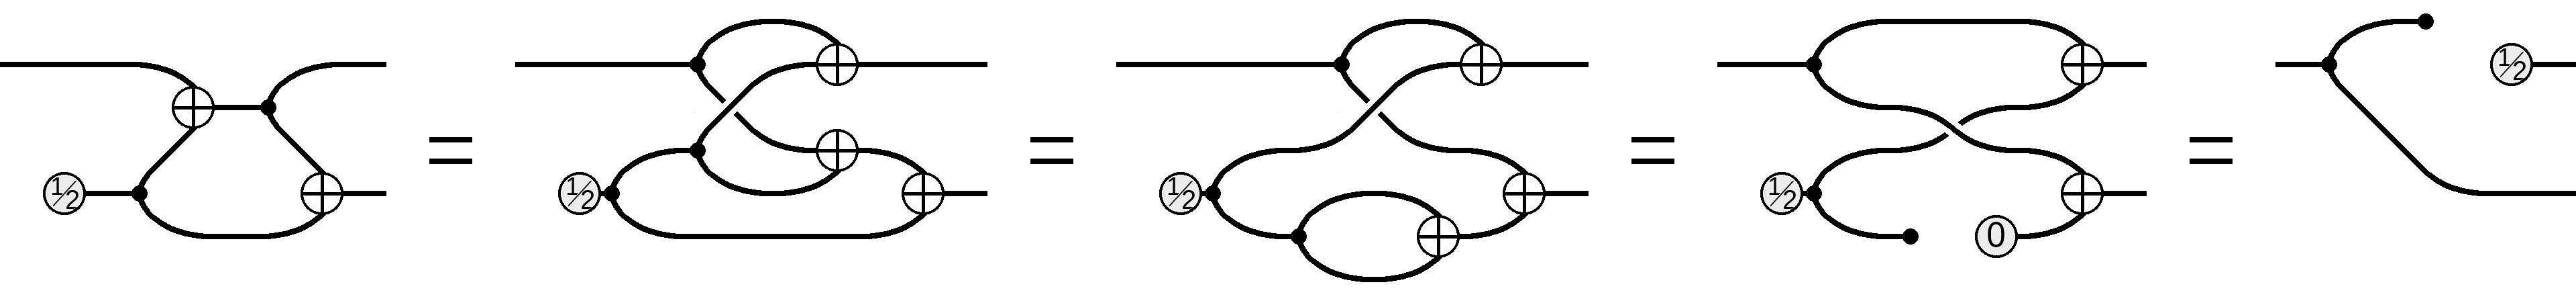
\includegraphics[height=28.125pt]{graphic-055.png}\end{matrix}$\par
 
The equations use the fact that $\oplus$ is deterministic, associative, idempotent, unitary with respect to $\langle 0\rangle$ and nullary with respect to $\langle\frac{1}{2}\rangle$. All of these properties can be proved via the axioms of Markov categories with probabilistic choice. For example the fact that $\langle\frac{1}{2}\rangle$ is absorbing for $\oplus$ is proved using the laws in Figure 2 as follows:\par
 
$\begin{matrix}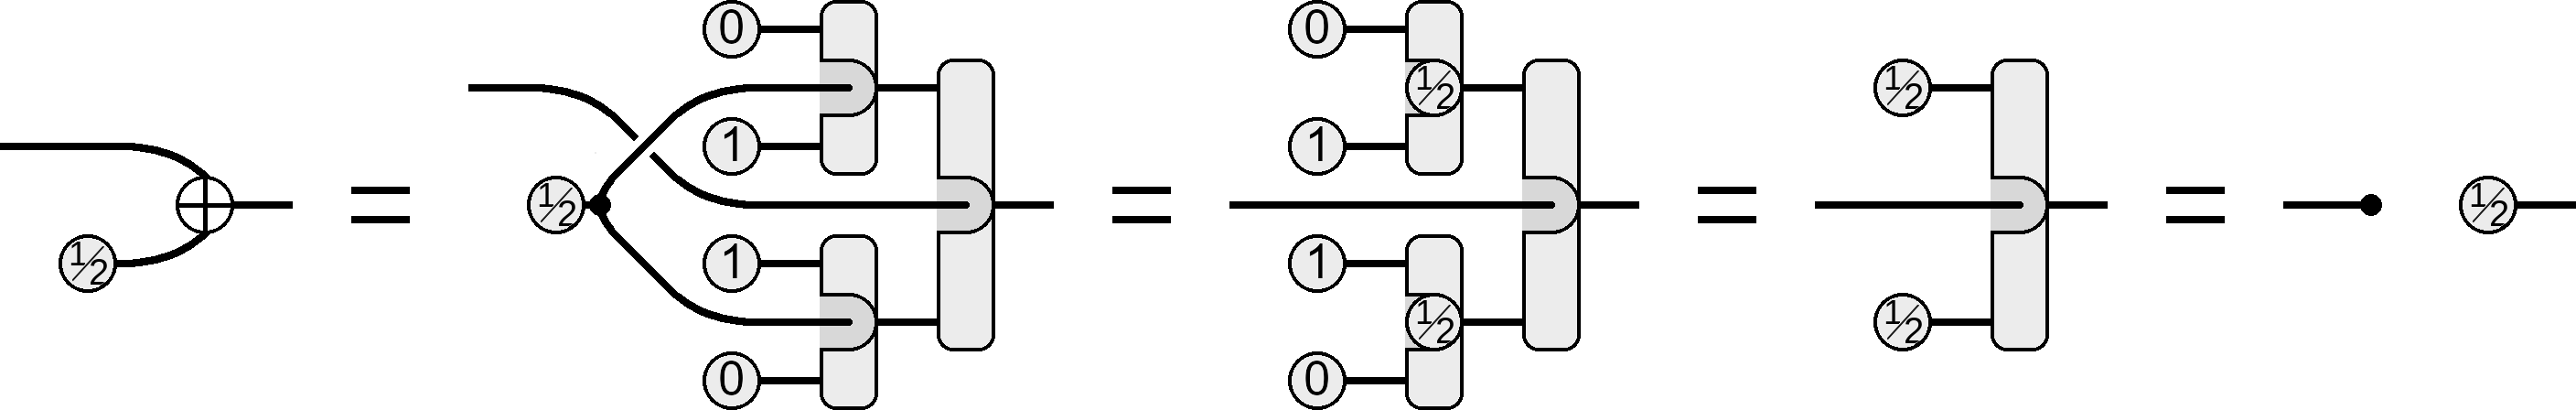
\includegraphics[height=28.125pt]{graphic-056.png}\end{matrix}$\par
 
% END S4.SS0.SSS0.P0.SPx1.p7
 
% BEGIN S4.SS0.SSS0.P0.SPx1.p8
 
Looking at $\textsf{PI}(\mathsf{FinStoch}_{\{1,0\}})$, the above example can be extended to operations on $\mathbb{B}^{\star}$, encrypting and decrypting $\star$-tuples of bits. We now show that the parametric iteration construction preserves the structure of Markov categories with probabilistic choice.\par
 
% END S4.SS0.SSS0.P0.SPx1.p8
 
% BEGIN Thmtheorem12
 
\par\medskip\noindent\textbf{Lemma 12.}\par
 
% BEGIN Thmtheorem12.p1
 
If $\mathcal{C}$ is a Markov category with probabilistic choice, then so is $\textsf{PI}(\mathcal{C})$.\par
 
% END Thmtheorem12.p1
 
% END Thmtheorem12
 
% END S4.SS0.SSS0.P0.SPx1
 
% BEGIN S4.SS0.SSS0.P0.SPx2
 
\par\medskip\noindent\textbf{Proof.}\par
 
% BEGIN S4.SS0.SSS0.P0.SPx2.p1
 
For $\mathbb{B}$ we can take $\llparenthesis\mathbb{B}\rrparenthesis$, and for $\langle p\rangle$ we take $\llparenthesis\langle p\rangle\rrparenthesis$. We define discard $!_{A\star}$, copy $\blacktriangleleft_{A\star}$ and case $\phi_{A^{\star}}$ for $\textsf{PI}(\mathcal{C})$ inductively on objects, with their definition on $A^{\star}$ being:\par
 
% END S4.SS0.SSS0.P0.SPx2.p1
 
% BEGIN S4.SS0.SSS0.P0.SPx2.p2
 
$\begin{matrix}
\includegraphics[height=4.375pt]{graphic-057.png}\end{matrix}$ := $\begin{matrix}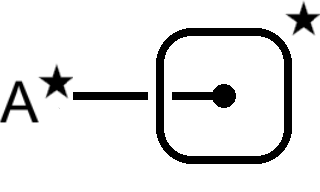
\includegraphics[height=12.5pt]{graphic-058.png}\end{matrix}$ $\begin{matrix}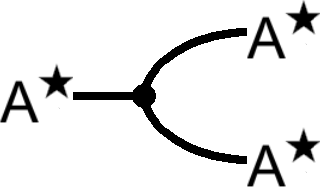
\includegraphics[height=12.5pt]{graphic-059.png}\end{matrix}$ := $\begin{matrix}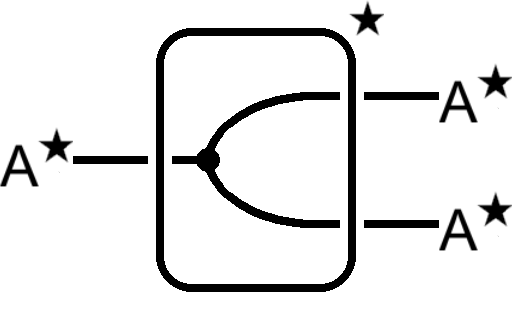
\includegraphics[height=20.0pt]{graphic-060.png}\end{matrix}$ $\begin{matrix}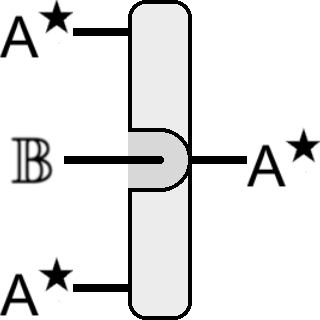
\includegraphics[height=20.0pt]{graphic-061.png}\end{matrix}$ := $\begin{matrix}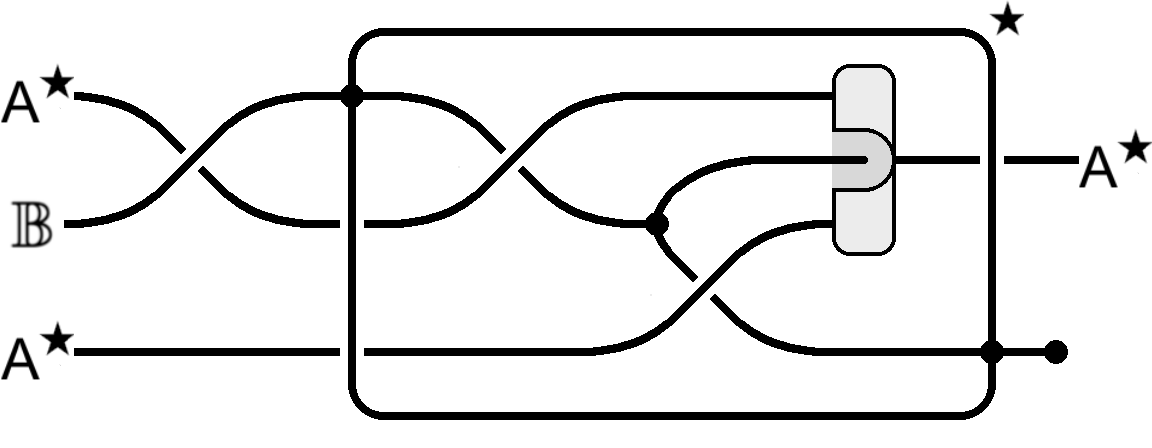
\includegraphics[height=28.125pt]{graphic-062.png}\end{matrix}$\par
 
% END S4.SS0.SSS0.P0.SPx2.p2
 
% BEGIN S4.SS0.SSS0.P0.SPx2.p3
 
The relevant properties can be shown using the diagonal method, with the naturality equations in particular being instances of Newton’s cradle. $\hfill\blacktriangleleft$\par
 
% END S4.SS0.SSS0.P0.SPx2.p3
 
% END S4.SS0.SSS0.P0.SPx2
  
% END S4


% BEGIN A2
 
\par\medskip\noindent\textbf{Appendix B A Complete Equational Theory of Boolean Stochastic Maps}\par
 
% BEGIN A2.p1
 
The structure of Markov categories with probabilistic choice, introduced in Section 4, is novel. Thus, it is interesting to study whether the axioms are complete with respect to the category $\mathsf{FinStoch}_{\{1,0\}}$. Here, completeness means that any equality between Boolean stochastic maps in $\mathsf{FinStoch}_{\{1,0\}}$ can also be derived syntactically using the axioms listed in Figure 1.\par
 
% END A2.p1
 
% BEGIN A2.p2
 
In order to formally state completeness, we introduce the syntactic category $\mathsf{PBCirc}$ of probabilistic boolean circuits. This is the symmetric monoidal category of string diagrams freely generated by the single-sorted signature $(\mathbb{B},\Sigma)$, where $\Sigma:=\{\begin{matrix}
\includegraphics[height=4.375pt]{graphic-063.png}\end{matrix},\begin{matrix}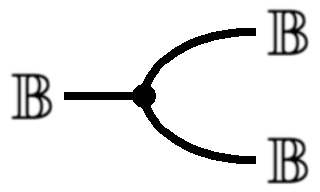
\includegraphics[height=12.5pt]{graphic-064.png}\end{matrix},\begin{matrix}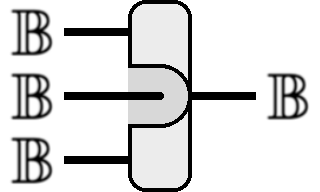
\includegraphics[height=12.5pt]{graphic-065.png}\end{matrix},\begin{matrix}
\includegraphics[height=4.375pt]{graphic-066.png}\end{matrix}\}$ and such that the morphisms are quotiented by the axioms in Figure 1.\par
 
% END A2.p2
 
% BEGIN A2.p3
 
Diagrams in $\mathsf{PBCirc}$ take semantics in $\mathsf{FinStoch}_{\{1,0\}}$ via the interpretation functor $\llbracket-\rrbracket\colon$ ${\mathsf{PBCirc}\to\mathsf{FinStoch}_{\{1,0\}}}$, defined inductively as follows:\par
  
\par  \quad  \[\llbracket\mathbb{B}\rrbracket:=\{1,0\}\quad\llbracket\begin{matrix}
\includegraphics[height=4.375pt]{graphic-063.png}\end{matrix}\rrbracket:=!_{\{1,0\}}\quad\llbracket\begin{matrix}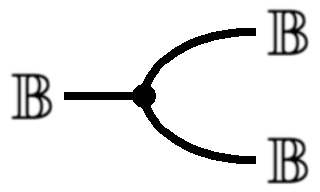
\includegraphics[height=12.5pt]{graphic-064.png}\end{matrix}\rrbracket:=\blacktriangleleft_{\{1,0\}}\quad\llbracket\begin{matrix}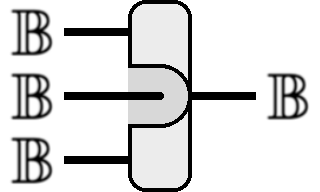
\includegraphics[height=12.5pt]{graphic-065.png}\end{matrix}\rrbracket:=\phi_{\{1,0\}}\quad\llbracket\begin{matrix}
\includegraphics[height=4.375pt]{graphic-066.png}\end{matrix}\rrbracket:=\langle p\rangle\]\quad  \quad  
  
Then we say that the equational theory of $\mathsf{PBCirc}$ is complete for $\mathsf{FinStoch}_{\{1,0\}}$ if, for any two diagrams $c,d\in\mathsf{PBCirc}$ of the same type, if $\llbracket c\rrbracket=\llbracket d\rrbracket$ then their equality can be derived using the axioms in Figure 1. We rephrase Theorem 11.\par
 
% END A2.p3
 

% BEGIN Thmtheorem23
 
\par\medskip\noindent\textbf{Theorem 23.}\par
 
% BEGIN Thmtheorem23.p1
 
The equational theory of $\mathsf{PBCirc}$ is complete for $\mathsf{FinStoch}_{\{1,0\}}$.\par
 
% END Thmtheorem23.p1
 
% END Thmtheorem23

 
% BEGIN A2.SS0.SSS0.P0.SPx1
 
\par\medskip\noindent\textbf{Proof.}\par
 
% BEGIN A2.SS0.SSS0.P0.SPx1.p1
 
The proof shows that each element of $\mathsf{FinStoch}_{\{1,0\}}$ has a unique normal form representation as a diagram in $\mathsf{PBCirc}$, and each diagram in $\mathsf{PBCirc}$ is provably equal to a diagram in normal form.\par
 
% END A2.SS0.SSS0.P0.SPx1.p1
 
% BEGIN A2.SS0.SSS0.P0.SPx1.p2
 
We first equip each set $\mathbb{B}^{n}$ with a linear order. We then say that a formal sum $p_{1}\cdot x_{1}+\dots+p_{m}\cdot x_{m}$ over $\mathbb{B}^{n}$ is in normal form if all $p_{i}>0$ and the list $x_{1},\dots,x_{m}$ forms a sorted list of elements without repetition. As such, a formal sum in normal form is either of the form $1\cdot x$, or $p\cdot x+(1-p)\cdot s$ with $p\in(0,1)$, and $s$ a formal sum in normal form, containing values $x^{\prime}$ all higher than $x$ according to the chosen order. Importantly, each distribution has a unique normal formal sum representation.\par
 
% END A2.SS0.SSS0.P0.SPx1.p2
 
% BEGIN A2.SS0.SSS0.P0.SPx1.p3
 
A weighted probabilistic tree over $\mathbb{B}^{n}$ is a diagram $I\to\mathbb{B}^{n}$ inductively defined as:\par
  
\par  \quad  \[t,r\quad:=\quad\langle b_{1}\rangle\otimes\dots\otimes\langle b_{n}\rangle\mid(t\otimes r);\phi^{p}_{\mathbb{B}^{n}}\]\quad  \quad  
  
where each $b_{i}\in\{0,1\}$. We represent a normal formal sum as a weighted probabilistic tree, by representing $1\cdot(b_{1},\dots,b_{n})$ as $\langle b_{1}\rangle\otimes\dots\otimes\langle b_{n}\rangle$, and $p\cdot(b_{1},\dots,b_{n})+(1-p)\cdot s$ as $(\langle b_{1}\rangle\otimes\dots\otimes\langle b_{n}\rangle\otimes t);\phi^{p}_{\mathbb{B}^{n}}$, where $t$ is the representation of the normal formal sum $s$. It can be shown that any weighted probabilistic tree over $\mathbb{B}^{n}$ is equal to the tree representation of a normal formal sum. This is done by using axioms ($\phi\text{-1}$), ($\phi\text{-co}$) and ($\phi\text{-as}$) to get rid of zero-probability branches, sorting the order, and re-associating branches, as well as determinism of $\langle 1\rangle$, $\langle 0\rangle$ combined with ($\phi\text{-id}$) to combine branches with the same result.\par
 
% END A2.SS0.SSS0.P0.SPx1.p3
 
% BEGIN A2.SS0.SSS0.P0.SPx1.p4
 
The normal forms of type $\mathbb{B}^{0}\to\mathbb{B}^{n}$ are the tree representations of normal formal sums, which are unique for each distribution. We generalize to arbitrary $\mathbb{B}^{k}\to\mathbb{B}^{n}$ by doing a case distinction on inputs, where a normal form of type $\mathbb{B}^{k+1}\to\mathbb{B}^{n}$ is of the form: $(\blacktriangleleft_{\mathbb{B}^{k}}\otimes\textit{id}_{\mathbb{B}});(\textit{id}_{\mathbb{B}^{k}}\otimes\chi_{\mathbb{B}^{k},\mathbb{B}});(f_{1}\otimes\textit{id}_{\mathbb{B}}\otimes f_{0});\phi_{\mathbb{B}^{n}}$, where $f_{1}$ and $f_{0}$ are normal forms of morphisms of type $\mathbb{B}^{k}\to\mathbb{B}^{n}$. Each morphism $f:\mathbb{B}^{k}\multimap\mathbb{B}^{n}$ of $\mathsf{FinStoch}_{\{1,0\}}$ has a unique normal form of this kind, with $f:\mathbb{B}^{0}\to\mathbb{B}^{n}$ represented by the tree representation of the normal formal sum for the distribution given by $f(*)$, and $f:\mathbb{B}^{k+1}\to\mathbb{B}^{n}$ represented by taking $f_{1}$ and $f_{0}$ to be the normal form of the functions $(b_{1},\dots,b_{k})\mapsto f(b_{1},\dots,b_{k},1)$ and $(b_{1},\dots,b_{k})\mapsto f(b_{1},\dots,b_{k},0)$ respectively. This normal form is unique, as this specification is necessitated by the $\llbracket-\rrbracket$ functor.\par
 
% END A2.SS0.SSS0.P0.SPx1.p4
 
% BEGIN A2.SS0.SSS0.P0.SPx1.p5
 
See below examples of normal forms, with a normal form of a morphism of type $\mathbb{B}^{0}\to\mathbb{B}^{3}$ on the left in the form of a sorted weighted tree (using lexicographic ordering on $\mathbb{B}^{3}$), and a normal form of a morphism of type $\mathbb{B}^{3}\to\mathbb{B}^{k}$ with a weighted tree at each $t$ (some liberties were taken regarding the order of swaps and copies).\par
 
$\begin{matrix}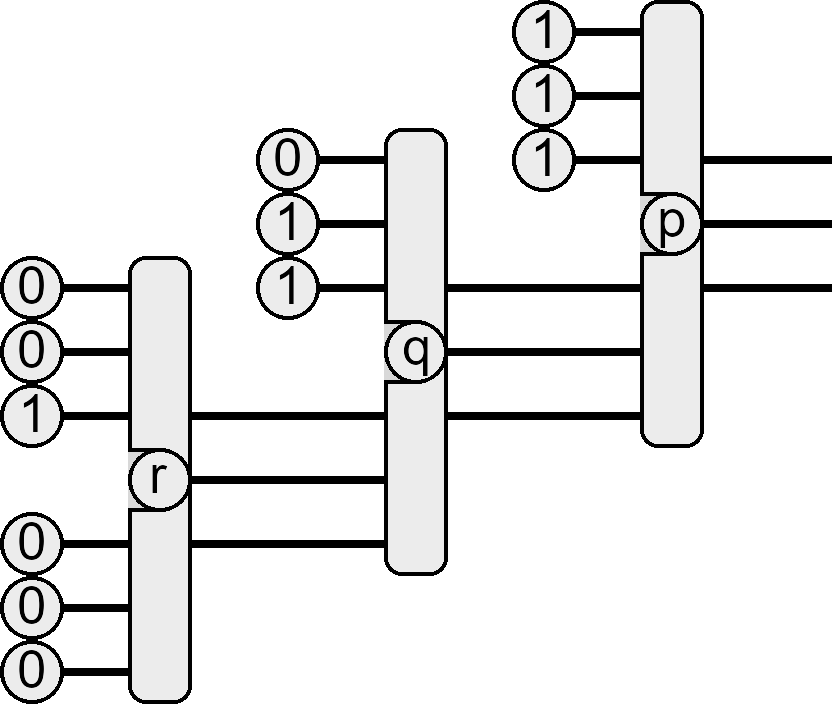
\includegraphics[height=44.375pt]{graphic-067.png}\end{matrix}$ $\begin{matrix}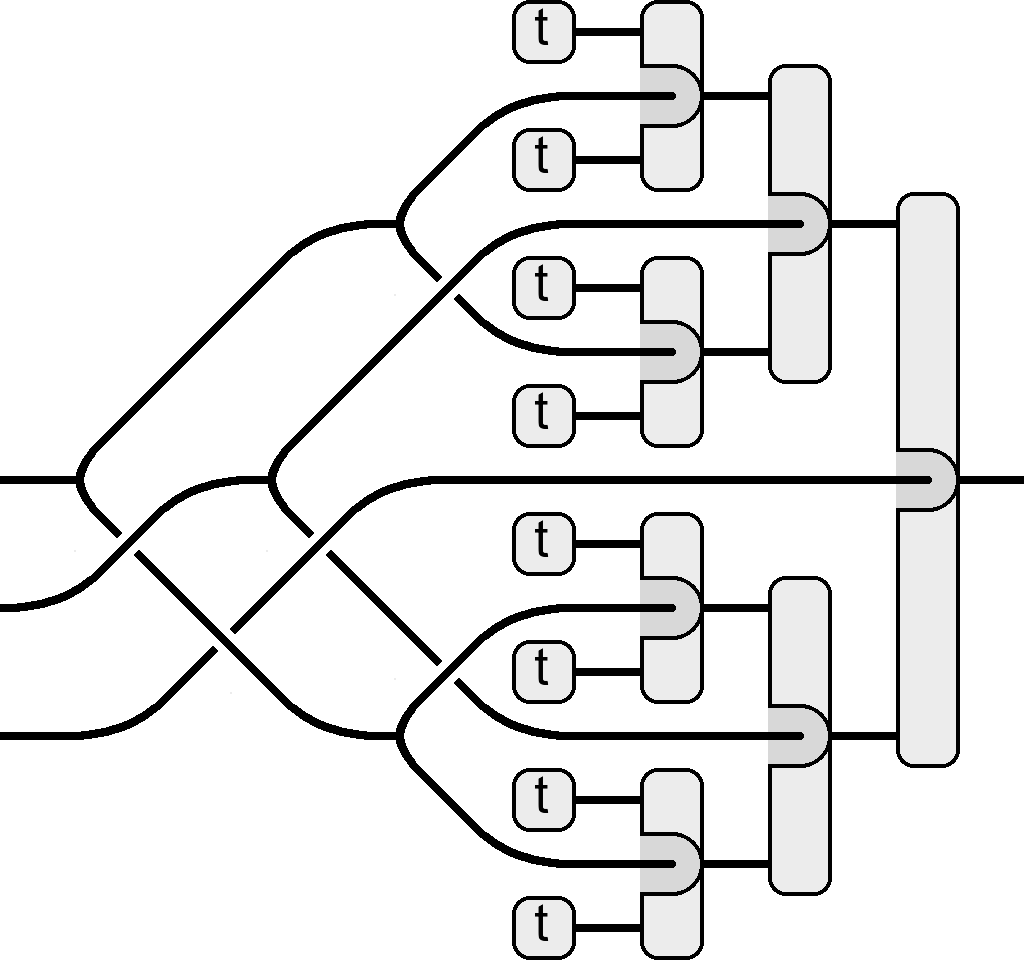
\includegraphics[height=60.0pt]{graphic-068.png}\end{matrix}$\par
 
% END A2.SS0.SSS0.P0.SPx1.p5
 
% BEGIN A2.SS0.SSS0.P0.SPx1.p6
 
We prove that each diagram is equivalent to one in normal form.\par
  
\par\noindent  $\blacksquare$ 
% BEGIN A2.I1.i1.p1
 
First we show that the identity diagrams $\textit{id}_{\mathbb{B}^{n}}:\mathbb{B}^{n}\to\mathbb{B}^{n}$ can be put in normal form. This can be shown by using the equations ($\phi\text{-B}$) and ($\phi\text{-id}$) together with monoidal coherence and naturality of $\phi$, given in equations ($\phi_I$), ($\phi_{\otimes}$), and ($\phi\text{-nat}$).\par
 
% END A2.I1.i1.p1
 
 
\par\noindent  $\blacksquare$ 
% BEGIN A2.I1.i2.p1
 
Second, note that each morphism in a freely generated monoidal category can be described as a composition of morphisms of the form $(\textit{id}_{A}\otimes s\otimes\textit{id}_{B})$, with $s$ a generator, which in our case is of $\{\chi\}\cup\Sigma=\{\chi,\blacktriangleleft,!,\langle p\rangle,\phi\}$. Then show that $f;(\textit{id}_{A}\otimes s\otimes\textit{id}_{B})$ can be reduced to a normal form, given that $f$ is in normal form. This is done in three steps:\par
  
\par\noindent  1. 
% BEGIN A2.I1.i2.I1.i1.p1
 
Pull $(\textit{id}_{A}\otimes s\otimes\textit{id}_{B})$ through each $\phi$ using naturality ($\phi\text{-nat}$), both the if-gates used to distinguish between different inputs, as well as the if-gates used in the weighted probabilistic trees, until we get to leaves of the trees.\par
 
% END A2.I1.i2.I1.i1.p1
 
 
\par\noindent  2. 
% BEGIN A2.I1.i2.I1.i2.p1
 
Reduce each $(\langle b_{1}\rangle\otimes\dots\otimes\langle b_{n}\rangle);(\textit{id}_{A}\otimes s\otimes\textit{id}_{B})$ to a weighted probabilistic tree.\par
 
% END A2.I1.i2.I1.i2.p1
 
 
\par\noindent  3. 
% BEGIN A2.I1.i2.I1.i3.p1
 
The result is $f$, but with different weighted probabilistic trees at each case in its case distinction. Put all those trees into normal form.\par
 
% END A2.I1.i2.I1.i3.p1
 
  
% END A2.I1.i2.p1
 
  
Hence we can normalize each $f:\mathbb{B}^{k}\to\mathbb{B}^{n}$ by first giving it a specification as composition of $(\textit{id}_{A}\otimes s\otimes\textit{id}_{B})$ morphisms. Then normalize the identity function on $\mathbb{B}^{k}$ and inductively normalize by composing with each additional layer. $\hfill\blacktriangleleft$\par
 
% END A2.SS0.SSS0.P0.SPx1.p6
 
% BEGIN Thmtheorem24
 
\par\medskip\noindent\textbf{Lemma 24.}\par
 
% BEGIN Thmtheorem24.p1
 
$\mathsf{PBCirc}$ is a metric enriched symmetric monoidal category.\par
 
% END Thmtheorem24.p1
 
% END Thmtheorem24
 
% END A2.SS0.SSS0.P0.SPx1


% BEGIN bib
 
\par\medskip\noindent\textbf{References}\par
  
\par\noindent  [1]  Filippo Bonchi, Cipriano Junior Cioffo, Alessandro Di Giorgio, and Elena Di Lavore.  Tape Diagrams for Monoidal Monads.  In Corina Cîrstea and Alexander Knapp, editors, 11th Conference on Algebra and Coalgebra in Computer Science (CALCO 2025), volume 342 of Leibniz International Proceedings in Informatics (LIPIcs), pages 11:1–11:24, Dagstuhl, Germany, 2025. Schloss Dagstuhl – Leibniz-Zentrum für Informatik.  doi:10.4230/LIPIcs.CALCO.2025.11.  
 
\par\noindent  [2]  Anne Broadbent and Martti Karvonen.  Categorical composable cryptography: extended version.  Logical Methods in Computer Science, Volume 19, Issue 4, December 2023.  doi:10.46298/lmcs-19(4:30)2023.  
 
\par\noindent  [3]  Ran Canetti.  Universally composable security: A new paradigm for cryptographic protocols.  In Proceedings 42nd IEEE Symposium on Foundations of Computer Science, pages 136–145. IEEE, 2001.  doi:10.1109/SFCS.2001.959888.  
 
\par\noindent  [4]  Titouan Carette, Dominic Horsman, and Simon Perdrix.  Szx-calculus: Scalable graphical quantum reasoning.  In MFCS 2019-44th International Symposium on Mathematical Foundations of Computer Science, volume 138, pages 55–1, 2019.  
 
\par\noindent  [5]  Apiwat Chantawibul and Pawel Sobocinski.  Monoidal multiplexing.  In B. Fischer and T. Uustalu, editors, Theoretical Aspects of Computing ? ICTAC 2018, volume 11187, pages 116–131. Springer, October 2018.  doi:10.1007/978-3-030-02508-3\_7.  
 
\par\noindent  [6]  Bob Coecke, Tobias Fritz, and Robert W Spekkens.  A mathematical theory of resources.  Information and Computation, 250:59–86, 2016.  doi:10.1016/J.IC.2016.02.008.  
 
\par\noindent  [7]  Cole Comfort, Antonin Delpeuch, and Jules Hedges.  Sheet diagrams for bimonoidal categories.  arXiv preprint arXiv:2010.13361, 2020.  
 
\par\noindent  [8]  Ugo Dal Lago, Furio Honsell, Marina Lenisa, and Paolo Pistone.  On Quantitative Algebraic Higher-Order Theories.  In Amy P. Felty, editor, 7th International Conference on Formal Structures for Computation and Deduction (FSCD 2022), volume 228 of Leibniz International Proceedings in Informatics (LIPIcs), pages 4:1–4:18, Dagstuhl, Germany, 2022. Schloss Dagstuhl – Leibniz-Zentrum für Informatik.  doi:10.4230/LIPIcs.FSCD.2022.4.  
 
\par\noindent  [9]  Elena Di Lavore, Giovanni de Felice, and Mario Román.  Monoidal streams for dataflow programming.  In Proceedings of the 37th Annual ACM/IEEE Symposium on Logic in Computer Science, LICS ’22, New York, NY, USA, 2022. Association for Computing Machinery.  doi:10.1145/3531130.3533365.  
 
\par\noindent  [10]  Tobias Fritz.  A synthetic approach to Markov kernels, conditional independence and theorems on sufficient statistics.  Advances in Mathematics, 370:107239, 2020.  arXiv:1908.07021.  
 
\par\noindent  [11]  Steven Holtzen, Guy Van den Broeck, and Todd Millstein.  Scaling exact inference for discrete probabilistic programs.  Proceedings of the ACM on Programming Languages, 4(OOPSLA):1–31, 2020.  doi:10.1145/3428208.  
 
\par\noindent  [12]  Nicholas Gauguin Houghton-Larsen.  A mathematical framework for causally structured dilations and its relation to quantum self-testing.  arXiv preprint arXiv:2103.02302, 2021.  arXiv:2103.02302.  
 
\par\noindent  [13]  André Joyal and Ross Street.  The geometry of tensor calculus, I.  Advances in Mathematics, 88(1):55–112, July 1991.  doi:10.1016/0001-8708(91)90003-P.  
 
\par\noindent  [14]  Jonathan Katz and Yehuda Lindell.  Introduction to Modern Cryptography, Second Edition.  Chapman \& Hall/CRC, 2nd edition, 2014.  
 
\par\noindent  [15]  A.N. Kolmogorov and S.V. Fomin.  Introductory Real Analysis.  Selected Russian publications in the mathematical sciences. Prentice-Hall, 1970.  URL: https://books.google.nl/books?id=9l4PAQAAMAAJ.  
 
\par\noindent  [16]  Ugo Dal Lago, Zeinab Galal, and Giulia Giusti.  On computational indistinguishability and logical relations.  In Programming Languages and Systems: 22nd Asian Symposium, APLAS 2024, Kyoto, Japan, October 22-24, 2024, Proceedings, pages 241–263, Berlin, Heidelberg, 2024. Springer-Verlag.  doi:10.1007/978-981-97-8943-6\_12.  
 
\par\noindent  [17]  Gabriele Lobbia, Wojciech Różowski, Ralph Sarkis, and Fabio Zanasi.  Quantitative Monoidal Algebra: Axiomatising Distance with String Diagrams.  In Paweł Gawrychowski, Filip Mazowiecki, and Michał Skrzypczak, editors, 50th International Symposium on Mathematical Foundations of Computer Science (MFCS 2025), volume 345 of Leibniz International Proceedings in Informatics (LIPIcs), pages 68:1–68:21, Dagstuhl, Germany, 2025. Schloss Dagstuhl – Leibniz-Zentrum für Informatik.  doi:10.4230/LIPIcs.MFCS.2025.68.  
 
\par\noindent  [18]  Saunders Mac Lane.  Categories for the Working Mathematician.  Springer, 1998.  
 
\par\noindent  [19]  Ueli Maurer.  Constructive cryptography–a new paradigm for security definitions and proofs.  In Joint Workshop on Theory of Security and Applications, pages 33–56. Springer, 2011.  doi:10.1007/978-3-642-27375-9\_3.  
 
\par\noindent  [20]  Ueli Maurer and Renato Renner.  Abstract cryptography.  In Bernard Chazelle, editor, Innovations in Computer Science - ICS 2011, Tsinghua University, Beijing, China, January 7-9, 2011. Proceedings, pages 1–21. Tsinghua University Press, 2011.  URL: http://conference.iiis.tsinghua.edu.cn/ICS2011/content/papers/14.html.  
 
\par\noindent  [21]  Robin Piedeleu, Mateo Torres-Ruiz, Alexandra Silva, and Fabio Zanasi.  A complete axiomatisation of equivalence for discrete probabilistic programming.  In Programming Languages and Systems: 34th European Symposium on Programming, ESOP 2025, Held as Part of the International Joint Conferences on Theory and Practice of Software, ETAPS 2025, Hamilton, ON, Canada, May 3–8, 2025, Proceedings, Part II, pages 202–229, Berlin, Heidelberg, 2025. Springer-Verlag.  doi:10.1007/978-3-031-91121-7\_9.  
 
\par\noindent  [22]  Robin Piedeleu and Fabio Zanasi.  An Introduction to String Diagrams for Computer Scientists.  Elements in Applied Category Theory. Cambridge University Press, 2025.  
 
\par\noindent  [23]  P. Selinger.  A Survey of Graphical Languages for Monoidal Categories, volume 813 of Lecture Notes in Physics, pages 289–355.  Springer, Berlin, Heidelberg, 2010.  doi:10.1007/978-3-642-12821-9\_4.  
 
\par\noindent  [24]  Mateo Torres-Ruiz, Robin Piedeleu, Alexandra Silva, and Fabio Zanasi.  On iteration in discrete probabilistic programming.  In 9th International Conference on Formal Structures for Computation and Deduction (FSCD 2024), volume 299 of Leibniz International Proceedings in Informatics (LIPIcs), pages 20:1–20:21. Schloss Dagstuhl – Leibniz-Zentrum für Informatik, 2024.  doi:10.4230/LIPIcs.FSCD.2024.20.  
  
% END bib

\end{document}
